% This is samplepaper.tex, a sample chapter demonstrating the
% LLNCS macro package for Springer Computer Science proceedings;
% Version 2.21 of 2022/01/12
%
\documentclass[runningheads]{llncs}
%
\usepackage[T1]{fontenc}
% T1 fonts will be used to generate the final print and online PDFs,
% so please use T1 fonts in your manuscript whenever possible.
% Other font encondings may result in incorrect characters.
%
\usepackage{graphicx}
\usepackage{amsmath}
\usepackage{algorithm}
\usepackage{algorithmic}
\usepackage{microtype}
\usepackage{hyphenat}
\usepackage{tikz}
\usetikzlibrary{arrows.meta,positioning,decorations.pathreplacing,patterns,calc}
\usepackage{xcolor}
%
%
% If you use the hyperref package, please uncomment the following two lines
% to display URLs in blue roman font according to Springer's eBook style:
%\usepackage{color}
%\renewcommand\UrlFont{\color{blue}\rmfamily}
%\urlstyle{rm}
%
\begin{document}
%
\title{Optimising Serverless Workflow Execution through Future-Based Execution, Partial Streaming and Intelligent Fusion}

\titlerunning{Optimising Serverless Workflow Execution}
%
%\titlerunning{Abbreviated paper title}
% If the paper title is too long for the running head, you can set
% an abbreviated paper title here
%
% \author{Harold-Nimrod Foldvari\inst{1}\orcidID{0009-0008-3531-0478} \and
% Daniel-George Malancioiu\inst{2}\orcidID{0009-0002-3210-9556} \and
% Mihai-Florin-Gabriel Craciun\inst{3}\orcidID{0000-0003-0335-8369}}
% %
% \authorrunning{N. Foldvari et al.}
% First names are abbreviated in the running head.
% If there are more than two authors, 'et al.' is used.
%
% \institute{Babes-Bolyai University, Cluj-Napoca, Romania}
%
\maketitle              % typeset the header of the contribution
%
\begin{abstract}
Serverless workflow orchestration suffers from cold-start serialisation in fan-in patterns and full-payload blocking between sequential functions; centralised orchestrators further amplify these costs. We present three novel enhancements to Unum~\cite{285171}, a decentralised orchestration framework: (i) \emph{future-based execution}, the first application of the futures abstraction from functional programming to serverless workflow orchestration, invokes fan-in aggregation early, overlapping cold-start initialisation with slower upstream branches; (ii) \emph{partial parameter streaming}, the first transfer of lazy-evaluation semantics to inter-function data flow, propagates each output field immediately, enabling downstream processing before full payload completion; and (iii) \emph{intelligent function fusion}, a novel hybrid pipeline that combines LLM-guided proposal generation with deterministic rule-based compiler validation, collapses eligible sequential chains into single deployment units at build time. On AWS Lambda workflows, these mechanisms reduce cold-start end-to-end latency by up to 51.2\%, warm-state latency by up to 47.2\%, and cost by up to 42.4\%, without modifying user code.


\keywords{Serverless Computing \and Workflow Orchestration \and Cold Start \and Function Fusion \and Latency Optimisation.}
\end{abstract}

\section{Introduction}
\label{sec:introduction}

Serverless computing has become a dominant paradigm for building cloud-native applications, with the global market growing from approximately \$3~billion in 2017 to an estimated \$25~billion in 2025~\cite{wen2022riseplanetserverlesscomputing,PrecedenceResearch2025}. As application complexity grows, serverless functions are increasingly composed into workflows that chain or parallelise individual function invocations.

Workflow execution, however, exposes two structural performance bottlenecks. First, serverless functions incur \emph{cold-start latency} when no warm environment is available~\cite{lin2019mitigatingcoldstartsserverless,shahrad2020serverless}; in multi-function workflows each function boundary is a potential cold-start point, and in fan-in patterns the aggregation function cannot be invoked until the slowest upstream branch completes. Second, functions today exchange \emph{fully materialised payloads}, forcing a downstream function to wait for its predecessor's complete output even when partial results would suffice. Section~\ref{sec:background} characterises these bottlenecks in detail.

Additionally, managed orchestration services such as AWS Step Functions introduce a \emph{centralised coordination overhead} that prior work has shown can increase end-to-end latency substantially~\cite{285171,285113}. Decentralised approaches, in which orchestration logic is co-located with user functions, eliminate this overhead but, as we show, still leave cold-start stalls and payload-blocking latency unaddressed.

We address these gaps with three novel contributions to Unum~\cite{285171}, a state-of-the-art decentralised serverless orchestration framework. To the best of our knowledge, these represent the first application of functional-programming abstractions---futures and lazy evaluation---as workflow-level optimisation mechanisms in serverless computing:
\begin{enumerate}\setlength{\itemsep}{1pt}
\item \emph{Future-based execution} (Section~\ref{sec:futures}): the first realisation of the futures abstraction~\cite{baker1977incremental,halstead1985multilisp} in serverless orchestration. The aggregation function is invoked as soon as the first upstream branch completes, overlapping its cold-start initialisation with slower branches.
\item \emph{Partial parameter streaming} (Section~\ref{sec:streaming}): the first transfer of lazy-evaluation semantics~\cite{hughes1989why} to inter-function data flow in serverless systems. Each computed output field is emitted immediately, and fields not yet available are represented using the same custom future type introduced for future-based execution, enabling the successor to begin processing before the full payload is ready.
\item \emph{Intelligent function fusion} (Section~\ref{sec:fusion}): a novel hybrid approach that combines LLM-guided proposal generation with deterministic compiler validation governed by a formally defined rule system~\cite{wurz2020migrating}.
\end{enumerate}
All three mechanisms preserve Unum's checkpoint-based exactly-once semantics and require no changes to user code. Evaluated on four representative AWS Lambda workflows, they reduce cold-start end-to-end latency by up to 51.2\%, warm-state latency by up to 47.2\%, and estimated cost by up to 42.4\% (Section~\ref{sec:evaluation}).


\section{Background and Motivation}
\label{sec:background}

\subsection{Unum and Decentralised Orchestration}

Unum~\cite{285171} is a decentralised serverless orchestration framework whose \texttt{unum-cli} compiler embeds continuation logic directly into each function at build time. Every function knows its successor and invokes it upon completion without consulting an external service. Intermediate outputs and synchronisation state are persisted to an intermediary data store, and a checkpoint mechanism ensures exactly-once execution. This architecture achieves up to $2\times$ faster execution and up to $9\times$ lower cost than AWS Step Functions~\cite{285171}.

\subsection{Functional Programming Origins}
\label{sec:fp-origins}

Two abstractions central to this work originate in functional and concurrent programming. \emph{Futures}~\cite{baker1977incremental,halstead1985multilisp} are placeholders for values being computed concurrently, created when a computation is spawned and \emph{forced} only when needed; Liskov and Shrira~\cite{liskov1988promises} extended them across address spaces with durability guarantees. \emph{Lazy evaluation}~\cite{hughes1989why} defers computation until a value is demanded, decoupling producers from consumers and enabling modular composition. In prior work~\cite{foldvari2025closer} we proposed integrating these constructs into serverless workflow execution; the present paper consolidates those ideas into concrete, evaluated implementations within the Unum framework.

\subsection{Structural Gaps in Workflow Execution}
\label{sec:gaps}

Even with decentralised orchestration, two workflow-level latency sources persist. Individual-function cold starts have been addressed through lightweight isolation~\cite{agache2020firecracker,du2020catalyzer}, container-pool management~\cite{fuerst2021faascache,lin2019mitigatingcoldstartsserverless}, and predictive warming~\cite{vahidinia2023rl}, but these target \emph{single-function} startup, not the \emph{compounding} across workflow boundaries.

We illustrate both gaps on the Monte Carlo Pipeline workflow (Figure~\ref{fig:baseline-gaps}), a diamond-topology DAG with seven functions.

\paragraph{Gap~1: Cold-Start Serialisation in Fan-In Patterns.}
At the fan-in point, the Aggregator cannot be invoked until both the slowest chain (Transform $\rightarrow$ Estimate $\rightarrow$ Validate, $\approx$4.8\,s) and the parallel Simulate branch ($\approx$1.2\,s) complete. The Aggregator's cold start~$C_s$ then executes \emph{after} the critical path, adding $C_s$ entirely to end-to-end latency. In general, for branches $B_1,\dots,B_n$ converging at aggregation function~$A$:
\begin{equation}
T_{\text{classic}} = \max_{1 \le i \le n} T(B_i) \;+\; C_s \;+\; T(A).
\label{eq:classic}
\end{equation}

\paragraph{Gap~2: Payload-Blocking Latency in Sequential Chains.}
Between Transform and Estimate---both in the critical chain---Estimate cannot begin until Transform's \emph{entire} output payload is ready, even though Transform produces multiple independent fields. For a producer~$f$ and consumer~$g$, the sequential latency is:
\begin{equation}
T_{\text{atomic}} = T_f + T_g,
\label{eq:atomic}
\end{equation}
with no overlap possible regardless of field independence.

\begin{figure}[t]
\centering
\resizebox{\textwidth}{!}{%
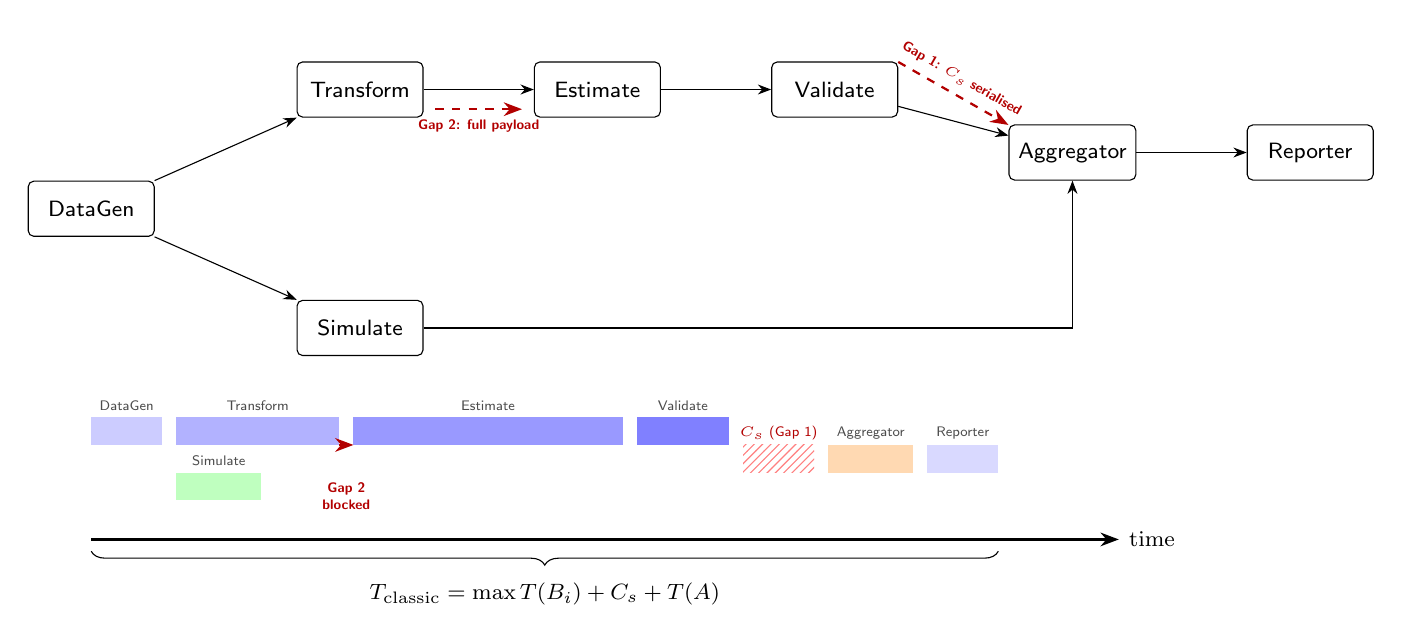
\begin{tikzpicture}[%
    >=Stealth,
    node distance=1.4cm and 1.8cm,
    fn/.style={rectangle, draw, rounded corners=2pt, minimum width=1.6cm, minimum height=0.7cm, font=\footnotesize\sffamily},
    gaparrow/.style={->, thick, red!70!black, dashed},
    timelabel/.style={font=\tiny\sffamily, text=black!70},
  ]
  % --- DAG (left) ---
  \node[fn] (dg) {DataGen};
  \node[fn, above right=0.8cm and 1.8cm of dg] (tr) {Transform};
  \node[fn, right=1.4cm of tr] (es) {Estimate};
  \node[fn, right=1.4cm of es] (va) {Validate};
  \node[fn, below right=0.8cm and 1.8cm of dg] (si) {Simulate};
  \node[fn, right=1.4cm of va, yshift=-0.8cm] (ag) {Aggregator};
  \node[fn, right=1.4cm of ag] (rp) {Reporter};

  \draw[->] (dg) -- (tr);
  \draw[->] (dg) -- (si);
  \draw[->] (tr) -- (es);
  \draw[->] (es) -- (va);
  \draw[->] (va) -- (ag);
  \draw[->] (si) -| (ag);
  \draw[->] (ag) -- (rp);

  % Gap annotations
  \draw[gaparrow] ($(va.east)+(0,0.35)$) -- ($(ag.west)+(0,0.35)$)
    node[midway, above, sloped, font=\tiny\sffamily\bfseries, text=red!70!black] {Gap~1: $C_s$ serialised};
  \draw[gaparrow] ($(tr.east)+(0.15,-0.25)$) -- ($(es.west)+(-0.15,-0.25)$)
    node[midway, below, font=\tiny\sffamily\bfseries, text=red!70!black] {Gap~2: full payload};

  % --- Timeline (right, below DAG) ---
  \begin{scope}[shift={(0,-4.2)}]
    \def\scale{0.9}
    \def\barh{0.35}

    % Axis
    \draw[->, thick] (0,0) -- (14.5*\scale,0) node[right, font=\footnotesize] {time};

    % Upper chain
    \fill[blue!20] (0,1.2) rectangle (1.0*\scale, 1.2+\barh);
    \node[timelabel] at (0.5*\scale, 1.2+\barh+0.15) {DataGen};

    \fill[blue!30] (1.2*\scale,1.2) rectangle (3.5*\scale, 1.2+\barh);
    \node[timelabel] at (2.35*\scale, 1.2+\barh+0.15) {Transform};

    \fill[blue!40] (3.7*\scale,1.2) rectangle (7.5*\scale, 1.2+\barh);
    \node[timelabel] at (5.6*\scale, 1.2+\barh+0.15) {Estimate};

    \fill[blue!50] (7.7*\scale,1.2) rectangle (9.0*\scale, 1.2+\barh);
    \node[timelabel] at (8.35*\scale, 1.2+\barh+0.15) {Validate};

    % Lower branch
    \fill[green!25] (1.2*\scale,0.5) rectangle (2.4*\scale, 0.5+\barh);
    \node[timelabel] at (1.8*\scale, 0.5+\barh+0.15) {Simulate};

    % Gap 1: Cold start serialised
    \fill[red!30, pattern=north east lines, pattern color=red!50] (9.2*\scale,0.85) rectangle (10.2*\scale, 0.85+\barh);
    \node[timelabel, text=red!70!black] at (9.7*\scale, 0.85+\barh+0.15) {$C_s$ (Gap~1)};

    % Aggregator
    \fill[orange!30] (10.4*\scale,0.85) rectangle (11.6*\scale, 0.85+\barh);
    \node[timelabel] at (11.0*\scale, 0.85+\barh+0.15) {Aggregator};

    % Reporter
    \fill[blue!15] (11.8*\scale,0.85) rectangle (12.8*\scale, 0.85+\barh);
    \node[timelabel] at (12.3*\scale, 0.85+\barh+0.15) {Reporter};

    % Gap 2: payload blocking
    \draw[gaparrow] (3.5*\scale,1.2) -- (3.7*\scale,1.2)
      node[midway, below=0.35cm, font=\tiny\sffamily\bfseries, text=red!70!black, align=center] {Gap~2\\blocked};

    % Brace for total
    \draw[decorate, decoration={brace, amplitude=5pt, mirror}]
      (0,-0.15) -- (12.8*\scale,-0.15)
      node[midway, below=8pt, font=\footnotesize] {$T_{\text{classic}} = \max T(B_i) + C_s + T(A)$};
  \end{scope}
\end{tikzpicture}%
}%
\caption{Monte Carlo Pipeline: baseline workflow DAG (top) and execution timeline (bottom). \textbf{Gap~1}: the Aggregator's cold start~$C_s$ is serialised after the slowest branch. \textbf{Gap~2}: payload-blocking forces Estimate to wait for Transform's complete output. Red-hatched and dashed regions mark wasted latency.}
\label{fig:baseline-gaps}
\end{figure}

Futures and lazy evaluation---originally devised for concurrent functional programs---provide precisely the abstractions needed to eliminate these two serialisation points (Sections~\ref{sec:futures}--\ref{sec:streaming}). Section~\ref{sec:fusion} further eliminates function-boundary overhead via intelligent fusion.

\section{System Design and Implementation}
\label{sec:proposed_solution}
Figure~\ref{fig:extended-architecture} presents the extended architecture. The build-time layer comprises the \texttt{unum-cli} compiler, which translates a workflow definition into per-function configurations and now includes two additional passes: a streaming source transformation that injects field-level publication calls, and an intelligent fusion pass that collapses eligible sequential chains into single deployment units. The runtime layer is embedded inside every deployed function alongside user code and executes the \texttt{ingress}$\to$\texttt{user\_code}$\to$\texttt{egress} lifecycle; it is extended with future-based fan-in resolution and incremental field consumption. Both runtime mechanisms leverage the existing intermediary data store for checkpoint persistence, fan-in synchronisation, and lazy value resolution; checkpoint and continuation semantics remain unchanged.

\begin{figure}[t]
  \centering
  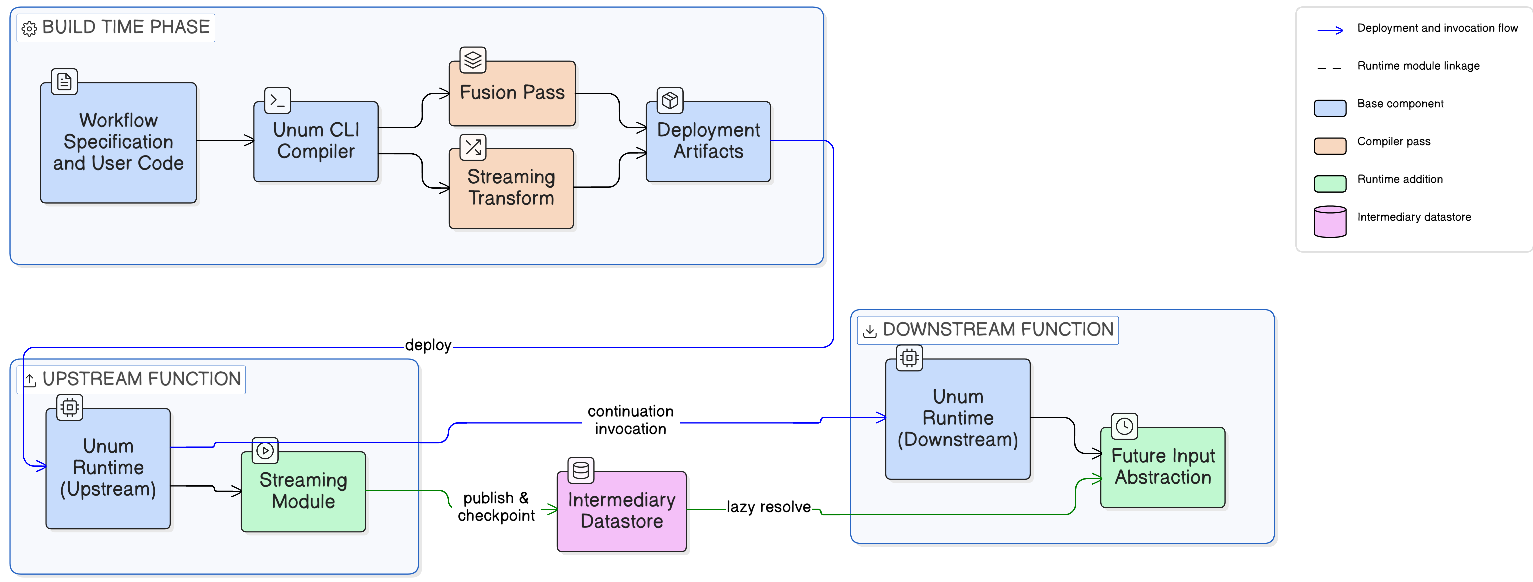
\includegraphics[width=\textwidth]{architecture.png}
  \caption{Extended Unum architecture. Build-time extensions (fusion, streaming transformation) augment the \texttt{unum-cli} compiler; runtime extensions (futures, incremental publication) are embedded alongside user functions.}
  \label{fig:extended-architecture}
\end{figure}

\subsection{Future-Based Execution}
\label{sec:futures}

Classical Unum fan-in requires all upstream branches to complete before invoking the aggregation function---the serverless equivalent of \emph{strict evaluation} (Section~\ref{sec:fp-origins}). We replace this with \emph{future-based} fan-in, applying the same future abstraction from functional programming: each unfinished branch's output is a future that resolves upon durable checkpoint creation, enabling the aggregation function to be invoked as soon as the \textbf{first} branch completes.

\paragraph{Latency Model.}
With future-based invocation, $A$ is invoked at $T_{\min}(B) = \min_{1 \le i \le n} T(B_i)$. Its cold start $C_s$ and initial execution then overlap with slower branches:
\begin{equation}
T_{\text{future}} = \max\!\bigl(\max_{1 \le i \le n} T(B_i),\;\; T_{\min}(B) + C_s + T(A)\bigr).
\label{eq:future}
\end{equation}
When $C_s + T(A) \le \max T(B_i) - T_{\min}(B)$, the cold start is \textbf{fully hidden}: $T_{\text{future}} = \max T(B_i)$. Figure~\ref{fig:futures-workflow} visualises the overlap against the baseline (Eq.~\ref{eq:classic}).

\paragraph{Early Invocation with Futures.}
Inputs to the aggregation function are a mixed vector of resolved values and futures:
\[
I_i =
\begin{cases}
o_i & \text{if } B_i \text{ has checkpointed (resolved)}, \\
F_i & \text{otherwise (future---forced on access)},
\end{cases}
\]
following the \emph{create--resolve--force} contract (Section~\ref{sec:fp-origins}): the runtime \emph{creates} a future at early invocation, a branch \emph{resolves} it upon checkpoint, and the aggregation function \emph{forces} it upon first access.

\paragraph{Runtime Mechanism.}
Language-native future and promise types (e.g., Python's \texttt{asyncio.Future}, JavaScript's \texttt{Promise}) cannot be used in this setting: inter-function payloads in serverless workflows must be fully serialisable for transmission through the intermediary data store, whereas language-level futures encapsulate in-process execution state and are inherently non-serialisable. We therefore introduce a custom \emph{datastore-backed future} type that is fully serialisable and resolution-transparent. Each future encapsulates either a resolved value or a pending reference keyed by invocation instance and branch identifier, exposing three operations: \emph{initialise} (allocate a durable placeholder in the data store), \emph{set\_value} (atomically write the resolved output and signal readiness), and \emph{await\_value} (suspend via efficient asynchronous polling with exponential back-off until the value materialises). Resolution occurs exclusively upon confirmed checkpoint creation, preserving exactly-once semantics. This custom future type is shared across both mechanisms presented in this section: future-based execution uses it at \emph{branch} granularity (Section~\ref{sec:futures}), while partial parameter streaming reuses it at \emph{field} granularity (Section~\ref{sec:streaming}).

\begin{figure}[t]
\centering
\resizebox{\textwidth}{!}{%
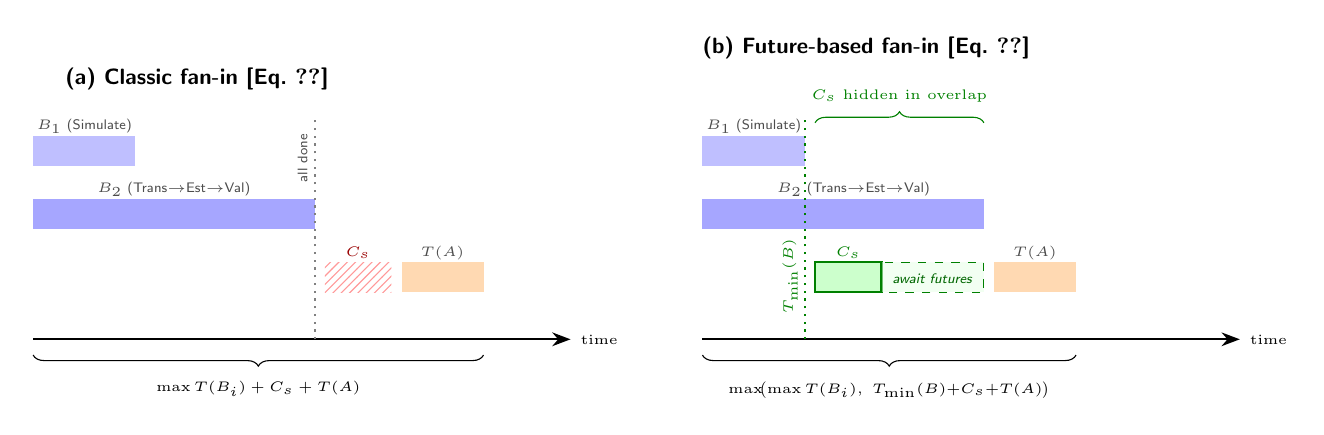
\begin{tikzpicture}[
    >=Stealth,
    timelabel/.style={font=\tiny\sffamily, text=black!70},
    eqlabel/.style={font=\scriptsize, text=black},
  ]
  \def\s{0.65}
  \def\barh{0.38}

  % ========= LEFT: CLASSIC =========
  \node[font=\footnotesize\bfseries\sffamily] at (3.2*\s, 3.3) {(a) Classic fan-in [Eq.~\ref{eq:classic}]};

  \draw[->, thick] (0,0) -- (10.5*\s,0) node[right, font=\tiny] {time};

  % Branches
  \fill[blue!25] (0, 2.2) rectangle (2*\s, 2.2+\barh);
  \node[timelabel] at (1*\s, 2.2+\barh+0.12) {$B_1$ (Simulate)};

  \fill[blue!35] (0, 1.4) rectangle (5.5*\s, 1.4+\barh);
  \node[timelabel] at (2.75*\s, 1.4+\barh+0.12) {$B_2$ (Trans$\to$Est$\to$Val)};

  % wait line
  \draw[dotted, thick, gray] (5.5*\s, 0) -- (5.5*\s, 2.8);
  \node[timelabel, rotate=90, anchor=south] at (5.55*\s, 2.3) {all done};

  % Cold start
  \fill[red!25, pattern=north east lines, pattern color=red!40] (5.7*\s, 0.6) rectangle (7.0*\s, 0.6+\barh);
  \node[timelabel, text=red!60!black] at (6.35*\s, 0.6+\barh+0.12) {$C_s$};

  % Aggregator execution
  \fill[orange!30] (7.2*\s, 0.6) rectangle (8.8*\s, 0.6+\barh);
  \node[timelabel] at (8.0*\s, 0.6+\barh+0.12) {$T(A)$};

  % Brace
  \draw[decorate, decoration={brace, amplitude=4pt, mirror}]
    (0, -0.2) -- (8.8*\s, -0.2)
    node[midway, below=6pt, font=\tiny] {$\max T(B_i) + C_s + T(A)$};

  % ========= RIGHT: FUTURE-BASED =========
  \begin{scope}[shift={(8.5, 0)}]
  \node[font=\footnotesize\bfseries\sffamily] at (3.2*\s, 3.7) {(b) Future-based fan-in [Eq.~\ref{eq:future}]};

  \draw[->, thick] (0,0) -- (10.5*\s,0) node[right, font=\tiny] {time};

  % Branches
  \fill[blue!25] (0, 2.2) rectangle (2*\s, 2.2+\barh);
  \node[timelabel] at (1*\s, 2.2+\barh+0.12) {$B_1$ (Simulate)};

  \fill[blue!35] (0, 1.4) rectangle (5.5*\s, 1.4+\barh);
  \node[timelabel] at (2.95*\s, 1.4+\barh+0.12) {$B_2$   (Trans$\to$Est$\to$Val)};

  % Early invoke line
  \draw[dotted, thick, green!50!black] (2*\s, 0) -- (2*\s, 2.8);
  \node[timelabel, rotate=90, anchor=south, text=green!50!black] at (2.05*\s, 0.8) {$T_{\min}(B)$};

  % Cold start (overlapping)
  \fill[green!20] (2.2*\s, 0.6) rectangle (3.5*\s, 0.6+\barh);
  \draw[thick, green!50!black] (2.2*\s, 0.6) rectangle (3.5*\s, 0.6+\barh);
  \node[timelabel, text=green!50!black] at (2.85*\s, 0.6+\barh+0.12) {$C_s$};

  % Waiting region (overlap)
  \fill[green!10, opacity=0.5] (3.5*\s, 0.6) rectangle (5.5*\s, 0.6+\barh);
  \draw[dashed, green!50!black] (3.5*\s, 0.6) rectangle (5.5*\s, 0.6+\barh);
  \node[timelabel, text=green!40!black] at (4.5*\s, 0.6+0.17) {\textit{await futures}};

  % Aggregator execution
  \fill[orange!30] (5.7*\s, 0.6) rectangle (7.3*\s, 0.6+\barh);
  \node[timelabel] at (6.5*\s, 0.6+\barh+0.12) {$T(A)$};

  % Overlap brace
  \draw[decorate, decoration={brace, amplitude=4pt}, green!50!black]
    (2.2*\s, 2.75) -- (5.5*\s, 2.75)
    node[midway, above=4pt, font=\tiny, text=green!50!black] {$C_s$ hidden in overlap};

  % Total brace
  \draw[decorate, decoration={brace, amplitude=4pt, mirror}]
    (0, -0.2) -- (7.3*\s, -0.2)
    node[midway, below=6pt, font=\tiny] {$\max\!\bigl(\max T(B_i),\; T_{\min}(B){+}C_s{+}T(A)\bigr)$};
  \end{scope}
\end{tikzpicture}%
}%
\caption{Classic vs.\ future-based fan-in on the Monte Carlo Pipeline. (a)~In the classic model, $C_s$ and $T(A)$ are serialised after the slowest branch (Eq.~\ref{eq:classic}). (b)~With futures, $A$ is invoked at $T_{\min}(B)$; $C_s$ overlaps with slower branches and the aggregator awaits unresolved futures, yielding Eq.~\eqref{eq:future}. Green region marks the overlap that eliminates cold-start serialisation.}
\label{fig:futures-workflow}
\end{figure}


\subsection{Partial Parameter Streaming}
\label{sec:streaming}

Applying the lazy-evaluation principle (Section~\ref{sec:fp-origins}) to serverless outputs, we treat a function's structured return value as a \emph{lazy stream of fields}. Conventionally, consumer~$g$ cannot begin until producer~$f$ has finished \emph{every} field ($T_{\text{atomic}} = T_f + T_g$). Our approach publishes each field to the intermediary store as soon as it is computed; the downstream function is invoked after the first field with a mixed payload of resolved values and datastore-backed futures (Section~\ref{sec:futures}) for fields not yet available, resolved transparently via the same asynchronous polling mechanism.

\paragraph{Latency Model.}
Let~$f$ compute $m$ fields with per-field times $t_1^f, \dots, t_m^f$ and~$g$ process them with $t_1^g, \dots, t_m^g$. Expanding Equation~\eqref{eq:atomic} at field granularity: $T_{\text{atomic}} = \sum_{k=1}^{m} t_k^f + \sum_{k=1}^{m} t_k^g$.
With streaming, $g$ is invoked after the first field; its cold start~$C_s^g$ overlaps with $f$'s remaining computation:
\begin{equation}
T_{\text{stream}} = \max\!\Bigl(\sum_{k=1}^{m} t_k^f,\;\;\; t_1^f + C_s^g + \sum_{k=1}^{m} t_k^g\Bigr).
\label{eq:stream}
\end{equation}
When per-field times are balanced, this collapses to $T_{\text{stream}} \approx \max(T_f, T_g)$---\textbf{converting a sequential sum into a parallel maximum}. Figure~\ref{fig:streaming-workflow} visualises the overlap.

\paragraph{Build-Time Transformation.}
The \texttt{unum-cli} compiler injects streaming via static source transformation: for each field in a structured return, it identifies the computation site, inserts a publication call, and triggers early continuation after the first publication. Downstream functions lazily resolve future references upon access. Checkpointing remains unchanged.

\begin{figure}[t]
\centering
\resizebox{\textwidth}{!}{%
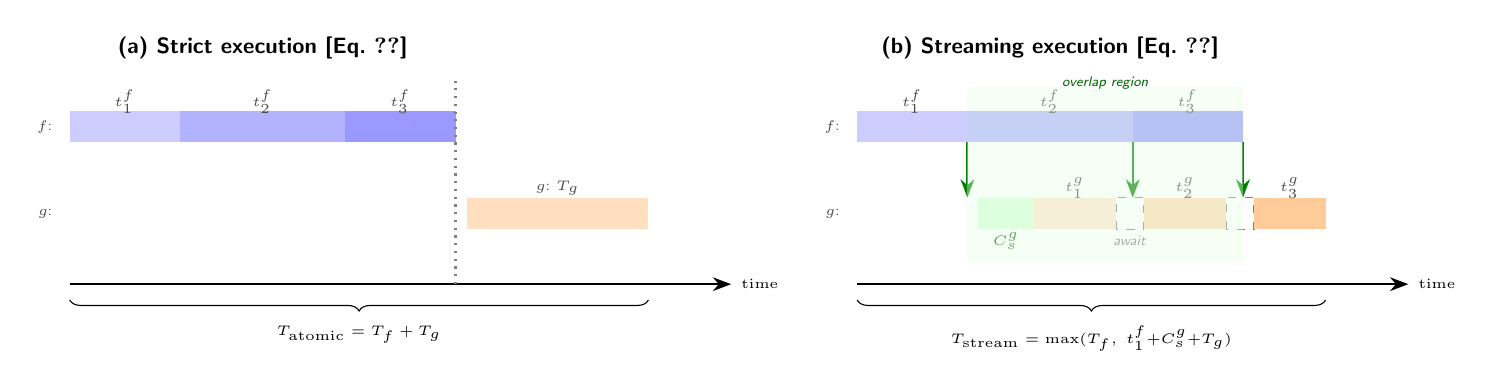
\begin{tikzpicture}[
    >=Stealth,
    timelabel/.style={font=\tiny\sffamily, text=black!70},
  ]
  \def\s{0.7}
  \def\barh{0.4}

  % ========= LEFT: STRICT =========
  \node[font=\footnotesize\bfseries\sffamily] at (3.5*\s, 3.0) {(a) Strict execution [Eq.~\ref{eq:atomic}]};

  \draw[->, thick] (0,0) -- (12*\s,0) node[right, font=\tiny] {time};

  % Producer fields
  \fill[blue!20] (0, 1.8) rectangle (2*\s, 1.8+\barh);
  \fill[blue!30] (2*\s, 1.8) rectangle (5*\s, 1.8+\barh);
  \fill[blue!40] (5*\s, 1.8) rectangle (7*\s, 1.8+\barh);
  \node[timelabel] at (1*\s, 1.8+\barh+0.12) {$t_1^f$};
  \node[timelabel] at (3.5*\s, 1.8+\barh+0.12) {$t_2^f$};
  \node[timelabel] at (6*\s, 1.8+\barh+0.12) {$t_3^f$};
  \node[timelabel, anchor=east] at (-0.1, 1.8+\barh/2) {$f$:};

  % Wait line
  \draw[dotted, thick, gray] (7*\s, 0) -- (7*\s, 2.6);

  % Consumer
  \fill[orange!25] (7.2*\s, 0.7) rectangle (10.5*\s, 0.7+\barh);
  \node[timelabel] at (8.85*\s, 0.7+\barh+0.12) {$g$: $T_g$};
  \node[timelabel, anchor=east] at (-0.1, 0.7+\barh/2) {$g$:};

  % Brace
  \draw[decorate, decoration={brace, amplitude=4pt, mirror}]
    (0, -0.2) -- (10.5*\s, -0.2)
    node[midway, below=6pt, font=\tiny] {$T_{\text{atomic}} = T_f + T_g$};

  % ========= RIGHT: STREAMING =========
  \begin{scope}[shift={(10, 0)}]
  \node[font=\footnotesize\bfseries\sffamily] at (3.5*\s, 3.0) {(b) Streaming execution [Eq.~\ref{eq:stream}]};

  \draw[->, thick] (0,0) -- (10*\s,0) node[right, font=\tiny] {time};

  % Producer fields
  \fill[blue!20] (0, 1.8) rectangle (2*\s, 1.8+\barh);
  \fill[blue!30] (2*\s, 1.8) rectangle (5*\s, 1.8+\barh);
  \fill[blue!40] (5*\s, 1.8) rectangle (7*\s, 1.8+\barh);
  \node[timelabel] at (1*\s, 1.8+\barh+0.12) {$t_1^f$};
  \node[timelabel] at (3.5*\s, 1.8+\barh+0.12) {$t_2^f$};
  \node[timelabel] at (6*\s, 1.8+\barh+0.12) {$t_3^f$};
  \node[timelabel, anchor=east] at (-0.1, 1.8+\barh/2) {$f$:};

  % Publish arrows
  \draw[->, thick, green!50!black] (2*\s, 1.8) -- (2*\s, 0.7+\barh);
  \draw[->, thick, green!50!black] (5*\s, 1.8) -- (5*\s, 0.7+\barh);
  \draw[->, thick, green!50!black] (7*\s, 1.8) -- (7*\s, 0.7+\barh);

  % Consumer fields
  \fill[green!15] (2.2*\s, 0.7) rectangle (3.2*\s, 0.7+\barh);
  \node[timelabel, text=green!40!black] at (2.7*\s, 0.7-0.15) {$C_s^g$};

  \fill[orange!20] (3.2*\s, 0.7) rectangle (4.7*\s, 0.7+\barh);
  \node[timelabel] at (3.95*\s, 0.7+\barh+0.12) {$t_1^g$};

  % Future ref (dashed until resolved)
  \draw[dashed, gray] (4.7*\s, 0.7) rectangle (5.2*\s, 0.7+\barh);
  \node[timelabel, text=gray] at (4.95*\s, 0.7-0.15) {\textit{await}};

  \fill[orange!30] (5.2*\s, 0.7) rectangle (6.7*\s, 0.7+\barh);
  \node[timelabel] at (5.95*\s, 0.7+\barh+0.12) {$t_2^g$};

  \draw[dashed, gray] (6.7*\s, 0.7) rectangle (7.2*\s, 0.7+\barh);
  \fill[orange!40] (7.2*\s, 0.7) rectangle (8.5*\s, 0.7+\barh);
  \node[timelabel] at (7.85*\s, 0.7+\barh+0.12) {$t_3^g$};
  \node[timelabel, anchor=east] at (-0.1, 0.7+\barh/2) {$g$:};

  % Overlap region
  \fill[green!10, opacity=0.4] (2*\s, 0.3) rectangle (7*\s, 2.5);
  \node[timelabel, text=green!40!black, font=\tiny\sffamily\itshape] at (4.5*\s, 2.55) {overlap region};

  % Brace
  \draw[decorate, decoration={brace, amplitude=4pt, mirror}]
    (0, -0.2) -- (8.5*\s, -0.2)
    node[midway, below=6pt, font=\tiny] {$T_{\text{stream}} = \max(T_f,\; t_1^f{+}C_s^g{+}T_g)$};
  \end{scope}
\end{tikzpicture}%
}%
\caption{Strict vs.\ streaming execution on a three-field producer--consumer pair (e.g., Estimate$\to$Validate in the Monte Carlo Pipeline). (a)~Strict: consumer waits for the full payload. (b)~Streaming: each field is published (green arrows) and consumed incrementally; dashed boxes mark future-reference awaits. The green shaded region shows the overlap that converts $T_f + T_g$ into $\approx \max(T_f, T_g)$.}
\label{fig:streaming-workflow}
\end{figure}

\subsection{Intelligent Function Fusion}
\label{sec:fusion}

Although future-based execution and partial streaming reduce synchronisation and data-propagation latency, sequential segments still incur structural overhead. We introduce an \emph{intelligent function fusion} mechanism that collapses eligible sequential chains into a single deployment unit at build time.

\paragraph{Latency Model.}

Consider a sequential scalar chain $F_1 \rightarrow F_2 \rightarrow \dots \rightarrow F_k$, where each function $F_i$ has execution time $T_i$ and cold-start overhead $C_s$. Under classical deployment:

\begin{equation}
T_{\text{chain}} = \sum_{i=1}^{k} (C_s + T_i).
\end{equation}

After fusion into a single function $F^{*}$:

\begin{equation}
T_{\text{fused}} = C_s + \sum_{i=1}^{k} T_i,
\end{equation}

since only one cold start is incurred and inter-function invocation overhead is eliminated. This formulation assumes that $C_s$ is dominated by runtime initialization and invocation setup rather than by modest increases in deployment package size. The benefit therefore grows with chain length and cold-start magnitude, motivating a rule-based mechanism that applies fusion only when correctness and efficiency are preserved.

\paragraph{Fusion Rule System.}

Fusion is governed by a rule system derived from the six structural migration principles for FaaS systems defined by W\"{u}rz et al.~\cite{wurz2020migrating}. Two functions are merged only when the first produces exactly one output consumed once by the second, forming a pure sequential link. Fusion cannot cross fan-in boundaries, entry-point functions remain isolated, and each function may appear in at most one fusion group. Table~\ref{tab:fusion-rules} summarises the six rules.

\begin{table}[t]
\caption{Fusion rule system derived from W\"{u}rz et al.~\cite{wurz2020migrating}.}
\label{tab:fusion-rules}
\centering
\small
\begin{tabular}{|c|l|l|}
\hline
\textbf{\#} & \textbf{Name} & \textbf{Constraint} \\
\hline
1 & Changing \# of elements & No fan-out/fan-in boundary crossing \\
2 & Alternative (OR-node) & Mutually exclusive branches stay separate \\
3 & Multiple uses & Shared callee not absorbed into one caller \\
4 & Varying resources & Memory difference $\le 2\times$ \\
5 & Long-running functions & Combined time $<$ platform max duration \\
6 & Too-different functions & Same runtime and team boundary \\
\hline
\end{tabular}
\end{table}

\paragraph{Hybrid Synthesis Pipeline.}

Candidate chains are identified by combining LLM-guided proposal generation with deterministic compiler validation. The compiler extracts workflow topology and per-function metadata (memory, timeout, runtime) from \texttt{unum-template.yaml} and \texttt{unum\_config.json}, and provides this context together with the fusion rules to the model. The LLM proposes fusion groups, but every proposal is validated against all six rules; only chains that pass deterministic checking are transformed---the compiler is the safety authority. Figure~\ref{fig:fusion-cli} illustrates this on the Smart Factory IoT workflow, where two eligible chains (MachineState$\rightarrow$ShiftCheck, Windowing$\rightarrow$ComputeFFT) are accepted while candidates crossing fan-in boundaries are rejected.

\begin{figure}[t]
  \centering
  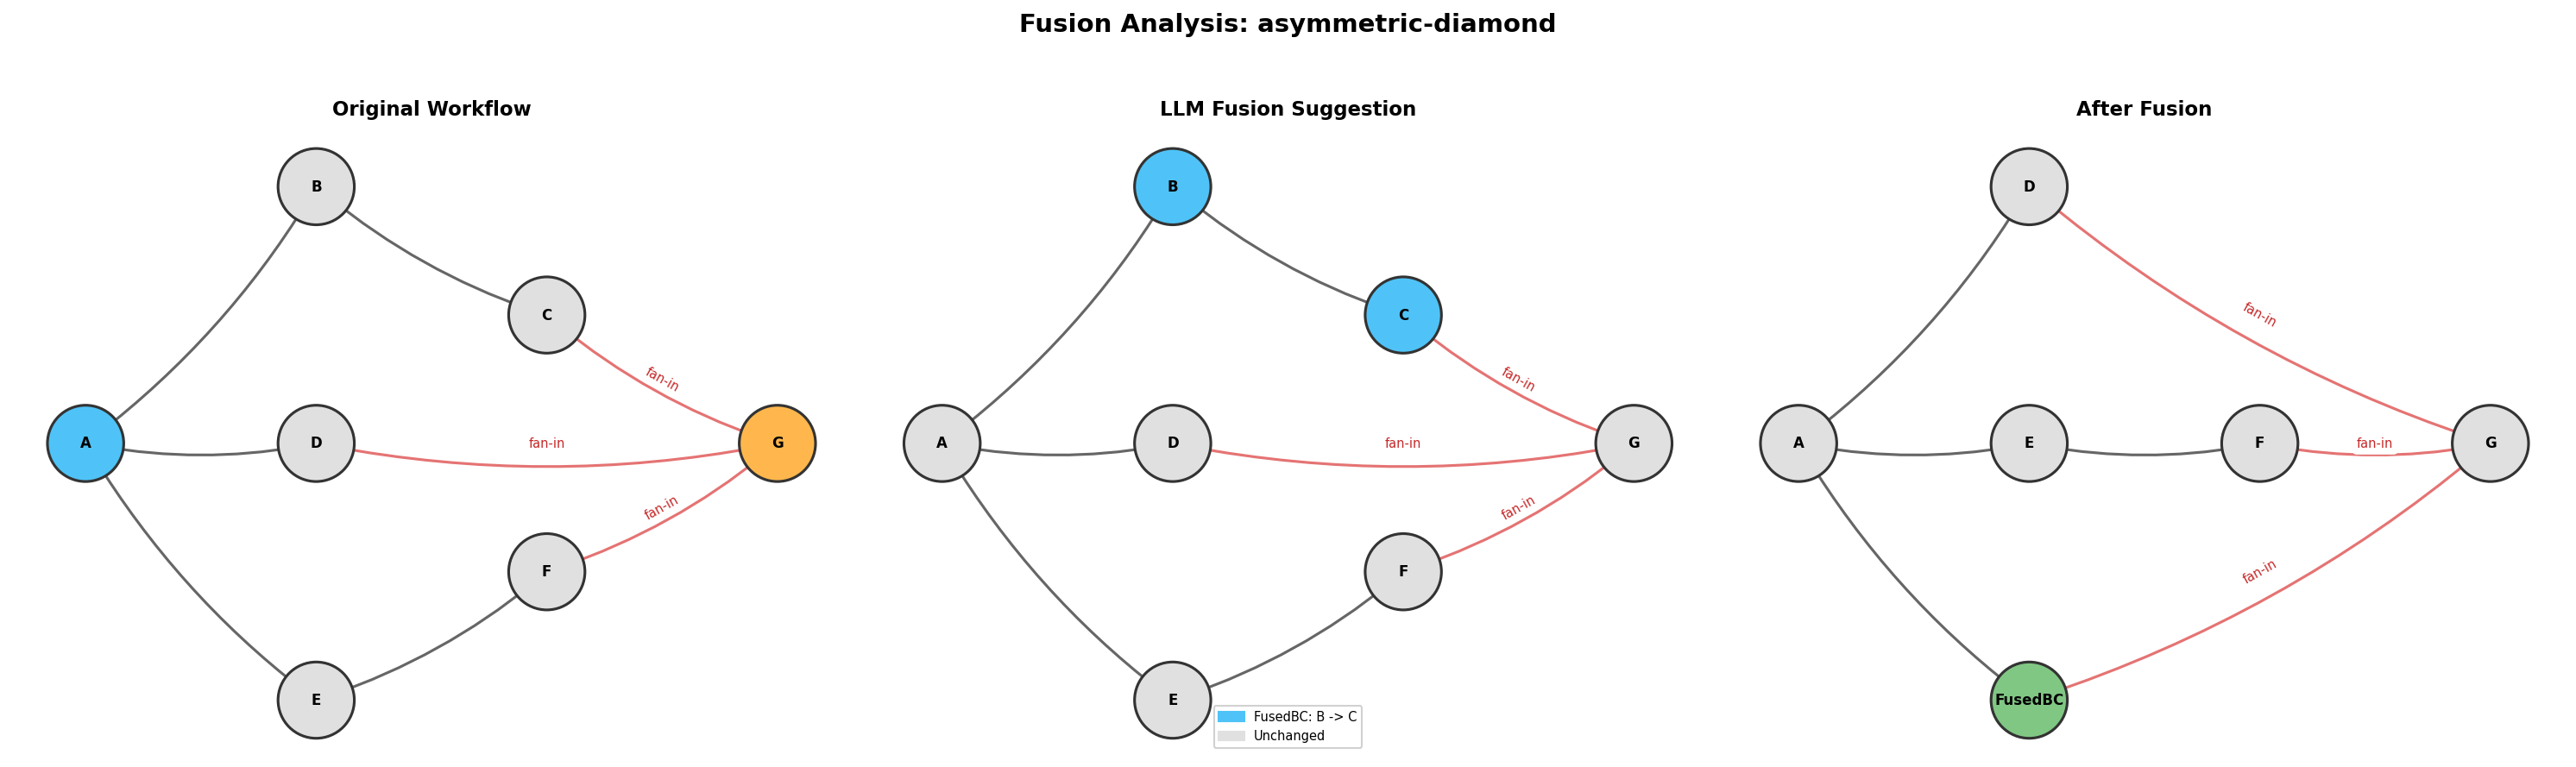
\includegraphics[width=\textwidth]{figures/fusion.png}
  \caption{\texttt{unum-cli fuse --ai} on the Smart Factory IoT workflow: the LLM proposes fusion candidates, explains rejections with rule references, and emits a \texttt{fusion.yaml} validated by the compiler.}
  \label{fig:fusion-cli}
\end{figure}

\paragraph{Code Generation and Template Rewriting.}

For each validated chain $F_1, \dots, F_k$, the compiler generates a fused function $F^{*}$:

\begin{algorithm}[t]
\caption{Generated Fused Handler}
\label{alg:fusion}
\begin{algorithmic}[1]
\STATE function fused\_handler(event, context)
\STATE \quad $x \leftarrow F_1(event, context)$
\FOR{$i = 2$ to $k$}
    \STATE \quad $x \leftarrow F_i(x, context)$
\ENDFOR
\STATE \quad return $x$
\end{algorithmic}
\end{algorithm}

The source code of each original function is preserved as an internal module. The workflow template is then rewritten such that incoming edges to $F_1$ are redirected to $F^{*}$, outgoing edges from $F_k$ originate from $F^{*}$, and intermediate functions are removed from deployment.

\paragraph{Semantic Preservation.}
All three mechanisms preserve exactly-once semantics under retry. Future resolution reads durably checkpointed values (idempotent on re-read). Streaming publication is keyed by instance and field name (idempotent on re-publish). Fusion replaces per-function checkpoints with a single boundary checkpoint at $F^{*}$; since no external component depends on intermediate state and continuation fires only after durable persistence, the fused unit is semantically equivalent to the original chain.



\section{Evaluation}
\label{sec:evaluation}

\subsection{Experimental Setup}

We evaluate on AWS Lambda (Python~3.11, 128\,MB, eu-central-1) with DynamoDB as the intermediary store, selecting four workflows that cover representative topologies with genuine computation. Crucially, all four correspond to workflow types widely used in serverless research and evaluation~\cite{eismann2021serverless}:
\begin{itemize}\setlength{\itemsep}{1pt}
\item \textbf{NLP Pipeline} (chain, 4~fn): Tokenizer$\to$Analyzer$\to$Classifier$\to$Summarizer; $\approx$12.7K-character input through tokenisation, NER, TF-IDF, and extractive summarisation. NLP inference pipelines are a well-established serverless use case~\cite{mankala2025nlp}.
\item \textbf{Text Processing} (fan-in, 5~fn): Two asymmetric branches (mention extraction, URL shortening) converging at post creation; from the original Unum app store~\cite{285171}.
\item \textbf{Monte Carlo Pipeline} (diamond, 7~fn): DataGen feeds a three-stage chain (Transform$\to$Estimate$\to$Validate) and a parallel Simulate branch, converging at Aggregator$\to$Reporter; 150$\times$150 matrix ops, 200K MC samples, Black-Scholes pricing. Monte Carlo simulation workflows are a standard benchmark for serverless scientific computing~\cite{hautz2023afcl,barcelona2022crucial}.
\item \textbf{Smart Factory IoT} (complex DAG, 8~fn): Sensor ingestion fans out to three branches (depth 1--3: safety, machine-state, FFT), converging at an action dispatcher. IoT data pipelines spanning edge-fog-cloud layers are a prominent serverless evaluation scenario~\cite{poojara2021iot}.
\end{itemize}
For each workflow we apply the enhancement best suited to its topology. Each is evaluated over 50~iterations (10~cold, 40~warm). Cold starts are forced by updating a Lambda environment variable and waiting 15\,s; two warm-up iterations are discarded. We report \emph{E2E latency}, \emph{billed duration}, and \emph{estimated cost} (Lambda + DynamoDB + S3, eu-central-1 pricing).

\begin{table}[t]
\caption{Evaluation results per workflow. $\Delta$\% is relative to the respective baseline.}
\label{tab:results}
\centering
\small
\begin{tabular}{|l|l|r|r|r|r|r|r|}
\hline
\textbf{Workflow} & \textbf{Config} & \textbf{Cold E2E} & \textbf{$\Delta$\%} & \textbf{Warm E2E} & \textbf{$\Delta$\%} & \textbf{Cost} & \textbf{$\Delta$\%} \\
 & & \textbf{(ms)} & & \textbf{(ms)} & & \textbf{(\$/1M exec.)} & \\
\hline
NLP Pipeline & Base    & 6,703  & ---     & 1,032  & ---      & 1.07  & ---     \\
             & Fusion  & 5,803  & $-13.4$ & 545    & $-47.2$  & 0.89  & $-16.8$ \\
\hline
Text Proc.   & Base    & 5,647  & ---     & 686    & ---      & 1.41  & ---     \\
             & Futures & 4,200  & $-25.6$ & 585    & $-14.7$  & 1.73  & $+22.7$ \\
\hline
Monte Carlo  & Base      & 12,591 & ---     & 5,345  & ---      & 2.97  & ---     \\
             & Futures   & 8,869  & $-29.6$ & 4,959  & $-7.2$   & 2.38  & $-19.9$ \\
             & Streaming & 9,154  & $-27.3$ & 4,604  & $-13.9$  & 2.77  & $-6.7$  \\
\hline
Smart Factory & Base     & 11,810 & ---     & 3,295  & ---      & 2.24  & ---     \\
IoT           & Futures  & 9,192  & $-22.2$ & 2,916  & $-11.5$  & 3.22  & $+43.8$ \\
              & Fusion   & 5,760  & $-51.2$ & 2,633  & $-20.1$  & 1.29  & $-42.4$ \\
\hline
\end{tabular}
\end{table}

\begin{figure}[t]
  \centering
  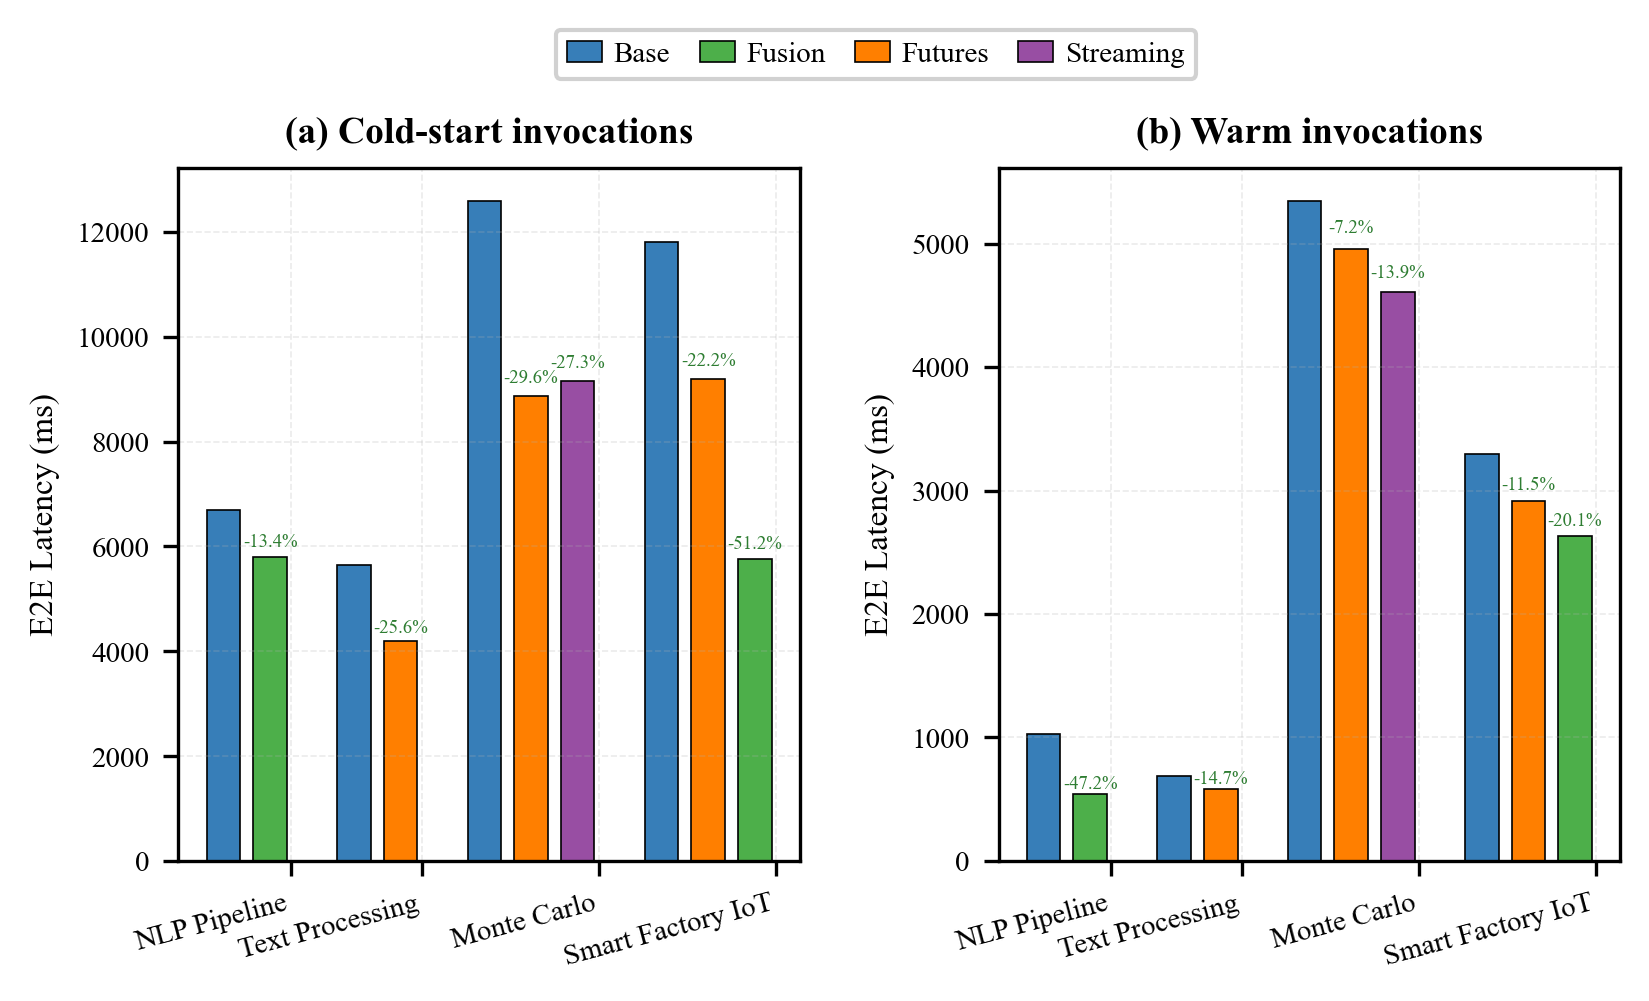
\includegraphics[width=\textwidth]{figures/fig_e2e_cold_warm.png}
  \caption{Cold-start (left) and warm (right) end-to-end latency for each workflow$\times$enhancement pair in Table~\ref{tab:results}. Percentage labels indicate change relative to baseline.}
  \label{fig:e2e}
\end{figure}
\subsection{Analysis by Enhancement}
\label{sec:analysis}

Table~\ref{tab:results} summarises the results across all configurations and Figure~\ref{fig:e2e} visualises end-to-end latency; we analyse each enhancement in turn.

\paragraph{Future-Based Execution.}
Futures overlap the aggregator's cold start with slower branch execution. On Text Processing, cold-start E2E decreases by \textbf{25.6\%}, validating Equation~\eqref{eq:future}; extended warm-state runs confirmed reductions up to \textbf{38.5\%}. On Monte Carlo (diamond topology), futures yield the largest cold-start reduction (\textbf{$-$29.6\%}): the compute-heavy Estimate function ($\approx$3,700\,ms) provides ample overlap time. On Smart Factory IoT, warm E2E falls by \textbf{11.5\%}, confirming generalisation to multi-branch topologies.

Futures introduce a cost increase on shallow DAGs (Text Processing $+$22.7\%, Smart Factory IoT $+$43.8\%) due to DynamoDB polling. On compute-dominated workflows (Monte Carlo) this overhead is fully amortised, yielding \textbf{simultaneous latency and cost reduction} ($-$19.9\%).

\paragraph{Partial Parameter Streaming.}
On Monte Carlo, streaming reduces cold-start E2E by \textbf{27.3\%} and warm E2E by \textbf{13.9\%}. On the NLP Pipeline with compute-intensive functions (Classifier: 3,215\,ms, Summarizer: 3,468\,ms), streaming achieves \textbf{$-$26.9\%} cold-start, \textbf{$-$18.6\%} warm, and a \textbf{98.8\% reduction in latency variance}. Streaming is most effective when per-field computation times substantially exceed intermediary-store write latency.

\paragraph{Intelligent Fusion.}
On the NLP Pipeline, collapsing three functions into one yields the \textbf{largest warm-state improvement ($-$47.2\%}), eliminating two Lambda invocations whose scheduling overhead dominates lightweight NLP.

On Smart Factory IoT, fusing two sequential pairs (MachineState$+$ShiftCheck, Windowing$+$ComputeFFT) reduces the topology from eight to six functions, achieving the \textbf{largest cold-start improvement ($-$51.2\%) and cost saving ($-$42.4\%)}. Compared with futures on the same workflow ($+$43.8\% cost), fusion reduces both latency \emph{and} cost by eliminating overhead rather than adding coordination. Fusion is the dominant optimisation when branch-internal sequential structure permits consolidation.


\section{Related Work}
\label{sec:related_work}

\paragraph{Serverless Workflow Orchestration.}
Data-centric systems such as Triggerflow~\cite{Arjona_2021}, Pheromone~\cite{285113,yu2025pheromone}, DataFlower~\cite{li2023dataflowerexploitingdataflowparadigm}, and DFlow~\cite{shi2023dflowefficientdataflowbasedinvocation} restructure orchestration around data availability. Decentralised approaches like Octopus~\cite{wang2025octopus} reduce scheduling overhead by up to $90\times$. Hybrid models~\cite{zhang2025federated,filinis2024intent} combine centralised and decentralised elements. Our mechanisms preserve Unum's continuation-based architecture and reduce latency \emph{within} it---complementing, rather than replacing, these directions.

\paragraph{Cold-Start Mitigation.}
Surveys~\cite{ebrahimi2024coldstart,golec2023coldstart} classify mitigation into checkpoint-restore (Catalyzer~\cite{du2020catalyzer}, SEUSS~\cite{cadden2020seuss}, SOCK~\cite{oakes2018sock}), predictive warming~\cite{vahidinia2023rl,hu2024predictive}, container-pool caching~\cite{fuerst2021faascache,yu2024rainbowcake}, and application-layer trimming (FaaSLight~\cite{liu2022faaslight}). All target \emph{single-function} cold starts. Our future-based execution and fusion address the \emph{workflow-level serialisation} of cold starts across function boundaries---a structural bottleneck these approaches leave unresolved.

\paragraph{Function Composition and Fusion.}
Lee et~al.~\cite{lee2021fusion} propose function fusion; workflow-aware scheduling~\cite{pan2024sustainable,quinn2021implications}, multi-cloud composition~\cite{elshamy2023orchestration,ristov2020afcl}, and co-schedu\-ling \cite{liu2025jointlambda} tackle related overhead. Our mechanism differs by coupling LLM-guided proposal with deterministic compiler validation and operating within a decentralised framework.

\paragraph{Limitations.}
Streaming is ineffective when per-field computation time is shorter than store-write latency. Futures on shallow DAGs can increase polling cost ($+43.8\%$ on Smart Factory IoT). Fusion misconfiguration is caught deterministically by the compiler. The evaluation is scoped to AWS Lambda with DynamoDB; generalisation remains future work.




\section{Conclusion}
\label{sec:conclusion}

We presented three extensions to Unum that shorten the critical path in decentralised serverless workflows by applying functional-programming abstractions---futures and lazy evaluation---to the serverless execution model: future-based execution overlaps aggregator cold starts with branch execution; partial streaming converts sequential payload handoff into parallel overlap; and intelligent fusion eliminates redundant cold starts in sequential chains. All three preserve exactly-once semantics without user-code changes, yielding cold-start latency reductions of up to \textbf{51.2\%}, warm-state reductions of up to \textbf{47.2\%}, and cost savings of up to \textbf{42.4\%} on AWS Lambda. Future work includes topology-aware automatic mechanism selection, multi-cloud generalisation, and integration with predictive cold-start mitigation.

% \begin{credits}
% \subsubsection{\discintname}
% The authors have no competing interests to declare that are relevant to the content of this article.
% \end{credits}
%
% ---- Bibliography ----
%
% BibTeX users should specify bibliography style 'splncs04'.
% References will then be sorted and formatted in the correct style.
%
\bibliographystyle{splncs04}
\bibliography{bibliography}
%
\end{document}
